\begin{frame}{Базовая работа с Git}{Изменение рабочей папки}
    \begin{columns}
        \begin{column}{0.6\textwidth}
            \begin{itemize}
                \item
                      Разрешается производить любые операции с файлами: добавлять новые, удалять старые, редактировать существующие
                \item
                      Текущее состояние рабочей папки можно проверить командой git status -- она должна показать измененные файлы.
                \item
                      Более подробный список изменений можно получить, используя команду git diff -- она покажет все изменения между рабочей папкой и индексом в каждом файле
            \end{itemize}
        \end{column}
        \begin{column}{0.4\textwidth}
            \begin{figure}
                \centering
                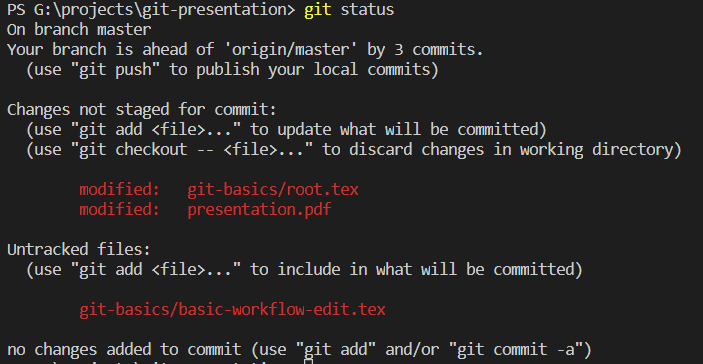
\includegraphics[width=\textwidth]{images/git-status-example.png}
                \caption{Пример git status}
            \end{figure}
            \begin{figure}
                \centering
                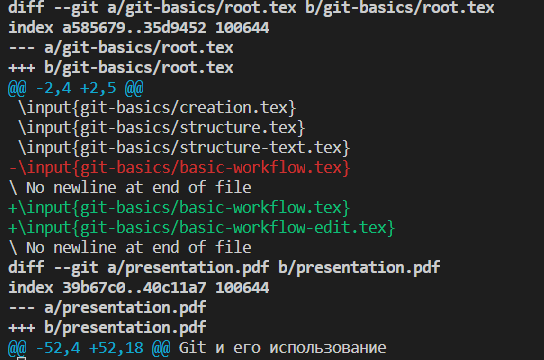
\includegraphics[width=\textwidth]{images/git-diff-example.png}
                \caption{Пример git diff}
            \end{figure}
        \end{column}
    \end{columns}

\end{frame}